\chapter{2. opgave}
Da vi tjekkede for outliers haved vi 12 kategorier at kigge på de er skrevet nedenfor i hvor tekst er skrevet til hver, givet om der er outliers eller ej.
\begin{enumerate}
\item Patient number id. \newline
De vil ikke give mening at lave en test da det er et nummer givet til dem 
\item  Time in study time.\\
\begin{figure}[H]
  \centering
  \begin{subfigure}[b]{0.49\textwidth}
    \includegraphics[width=\textwidth]{Basses_kode/Billeder_duration/Boxplot_of_ time .pdf}
    \caption{Boxplot over time}
    \label{fig:Residuals_plotted}
  \end{subfigure}
  \begin{subfigure}[b]{0.49\textwidth}
    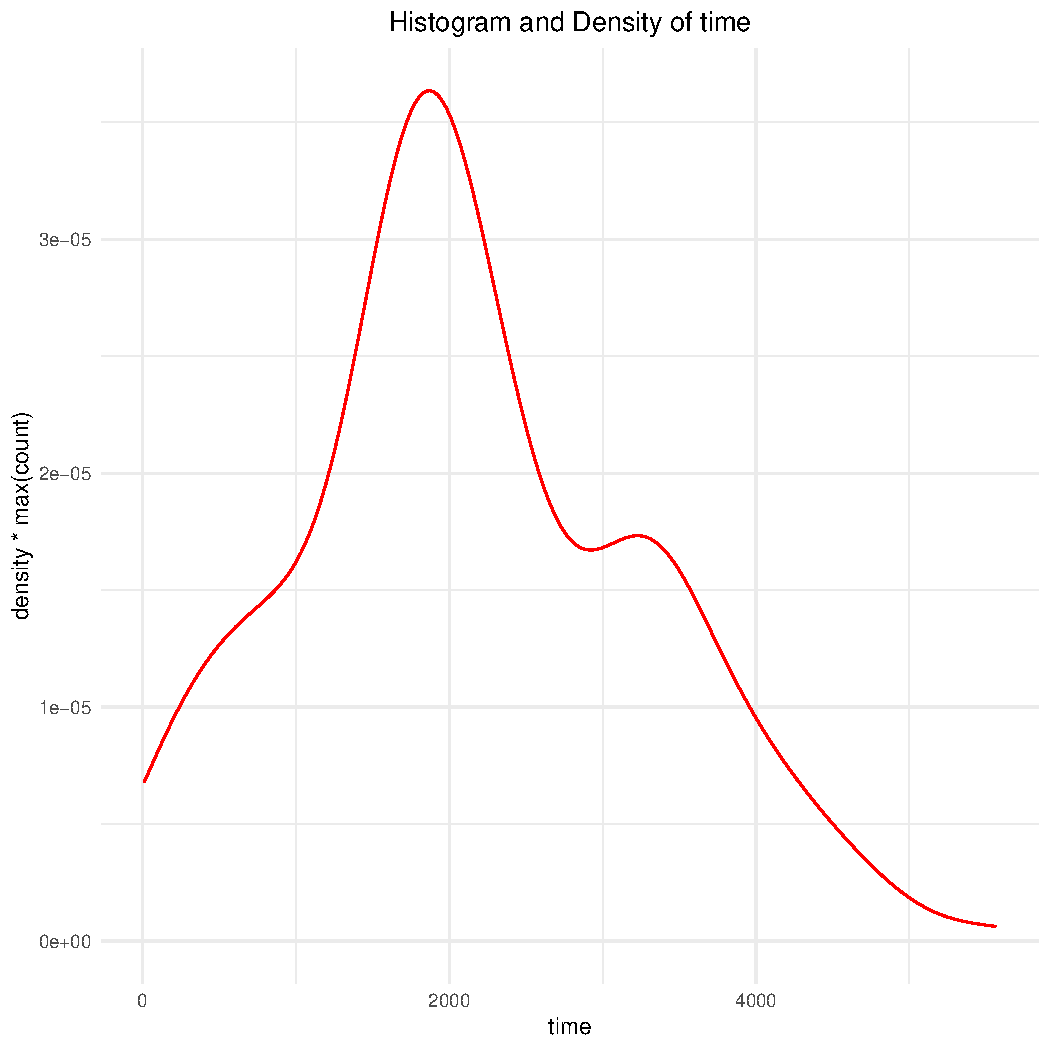
\includegraphics[width=\textwidth]{Basses_kode/Billeder_duration/Histogram_and_Density_of_ time .pdf}
    \caption{Density over time}
    \label{fig:long_ACF_residuals}
  \end{subfigure}
  \caption{Plots for outliers and density over time}
\end{figure}


\textbf{Outliers: }På billedet kan de ses at der er en enkel outlier, men siden det er en person der var i live i slutning må vi konkludere at det eneste der er at se er en rask patient der kom ind i forsøget tidligt.\\
\textbf{Distribution :} Plotter man densiteten af tidsgrafen ser man en nogenlunde normalfordeling dog med en, som forventet, tung højre hale


\item Cause of death status. \newline
\begin{table}[h]
    \centering
    \begin{tabular}{|l|c|c|c|}
        \hline
        & Alive 31 Dec 1977 & Dead from Malignant Melanoma & Dead from Other Cause \\
        \hline
        Count & 134 & 57 & 14 \\
        \hline
    \end{tabular}
    \caption{Summary of Cases by Status}
    \label{tab:summary}
\end{table}
Dette kan vi ikke rigtig kigge på outliers, da det er dødsårsagen 
\item Dead/alive at time of follow-up dead. \newline
\begin{table}[h!]
    \centering
    \begin{tabular}{|l|c|c|}
        \hline
        & Dead & Alive \\
        \hline
        Count & 134 & 71 \\
        \hline
    \end{tabular}
    \caption{Summary of Dead and Alive Cases}
    \label{tab:dead_alive}
\end{table}
Her kan vi Heller ikke kigge på outliers da det er status på patient efter et bestemt tids interval
\item Inflammatory cell infiltration score ici. \newline
\begin{table}[h!]
    \centering
    \begin{tabular}{|c|c|c|c|c|}
        \hline
        & 1 & 2 & 3 & 4 \\
        \hline
        Count & 17 & 59 & 107 & 22 \\
        \hline
    \end{tabular}
    \caption{Counts for Categories 1 to 4}
    \label{tab:categories}
\end{table}
\item Presence of epitheloid cells epicell. \newline
\begin{table}[h!]
    \centering
    \begin{tabular}{|l|c|c|}
        \hline
        Presence of Epitheloid Cells & No & Yes \\
        \hline
        Count & 116 & 89 \\
        \hline
    \end{tabular}
    \caption{Counts Based on Presence of Epitheloid Cells}
    \label{tab:epitheloid_cells}
\end{table}
\item Presence of ulceration ulceration. \newline
\begin{table}[h!]
    \centering
    \begin{tabular}{|l|c|c|}
        \hline
        Presence of Ulceration & No & Yes \\
        \hline
        Count & 115 & 90 \\
        \hline
    \end{tabular}
    \caption{Counts Based on Presence of Ulceration}
    \label{tab:ulceration}
\end{table}
\newpage
\item Thickness of tumor (1/100mm) thickness.

\begin{figure}[h]
    \centering
    \begin{subfigure}[b]{0.49\textwidth}
    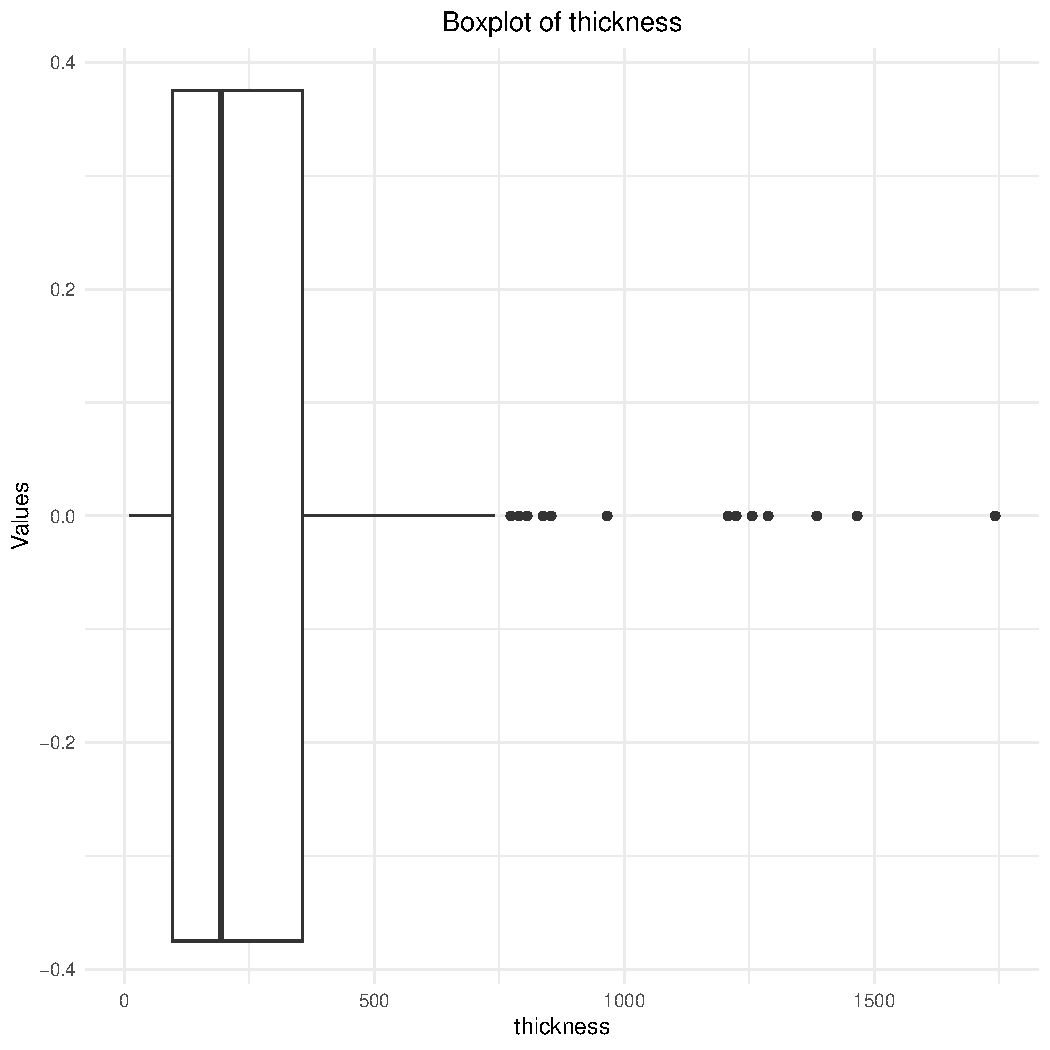
\includegraphics[width=\textwidth]{Basses_kode/Billeder_duration/Boxplot_of_ thickness .pdf}
    \end{subfigure}
    \begin{subfigure}[b]{0.49\textwidth}
    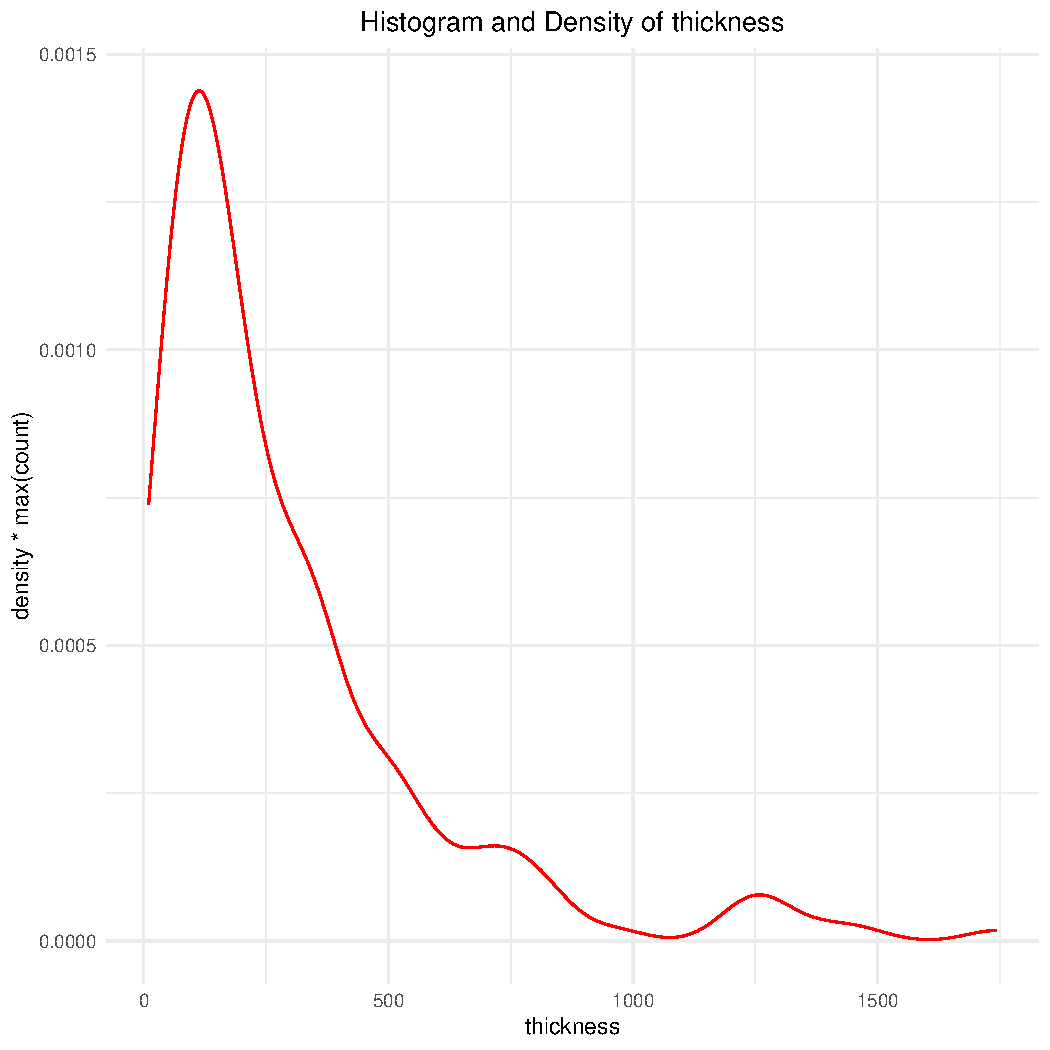
\includegraphics[width=\textwidth]{Basses_kode/Billeder_duration/Histogram_and_Density_of_ thickness .pdf}
    \end{subfigure}
\end{figure}
\textbf{Outliers:}Selvom vi ser mange Outliers, ved vi ikke om størrelsen har indflydelse på om patienten overlever eller ej, det bliver besvaret i næste opgave\\
\textbf{Distribution: } Tykkelsen af tumor fremstår som en betadistribution som er, naturligvis, ikke negativ, stiger i starten og falder derefter og får en lang højre hale. Undersøges yderligere logaritmen til disse værdier fremgår en nogenlunde normaldistribution.\\

\item Sex sex.\\
\begin{table}[h!]
    \centering
    \begin{tabular}{|l|c|c|}
        \hline
        Sex & Female & Male \\
        \hline
        Count & 126 & 79 \\
        \hline
    \end{tabular}
    \caption{Counts by Sex}
    \label{tab:sex}
\end{table}
\newpage
\item Age at operation age.
\newline
\begin{figure}[h]
    \centering
\begin{subfigure}[b]{0.49\textwidth}
    \includegraphics[width=\textwidth]{Basses_kode/Billeder_duration/Boxplot_of_ age .pdf}
    
\end{subfigure} 
\begin{subfigure}[b]{0.49\textwidth}
    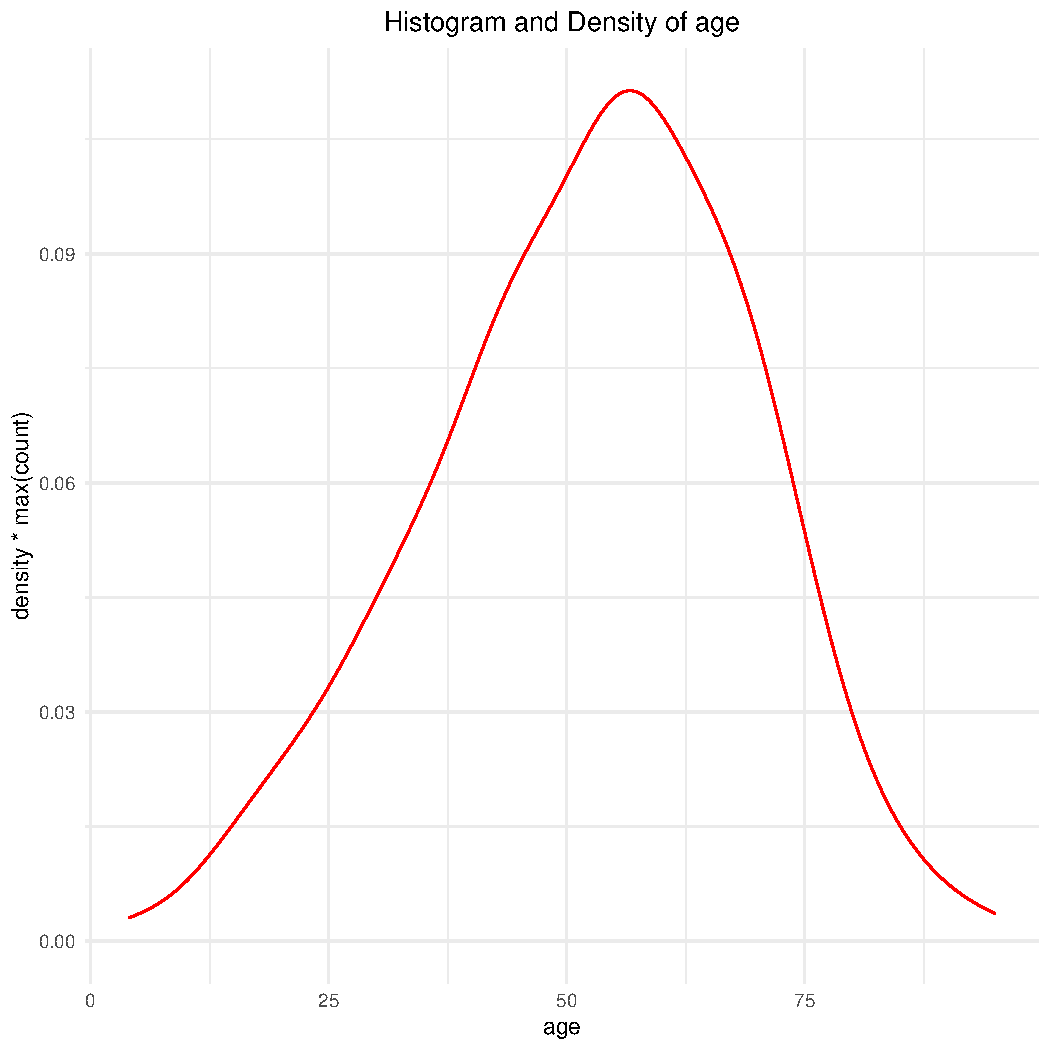
\includegraphics[width=\textwidth]{Basses_kode/Billeder_duration/Histogram_and_Density_of_ age .pdf}
\end{subfigure}  
\end{figure}

\textbf{Outliers: }Her ser vi en enkelt ung outlier 
\textbf{Age: } Aldersmæssigt haves en tung venstrehale og ellers fremstår en normal distribution nogenlunde
\newpage
\item Natural log of thickness/100 logthick.
\newline
\begin{figure}[h]
    \centering
    \begin{subfigure}[b]{0.49\textwidth}
    \includegraphics[width=\textwidth]{Basses_kode/Billeder_duration/Boxplot_of_ logthick .pdf}
    \end{subfigure}
    \begin{subfigure}[b]{0.49\textwidth}
    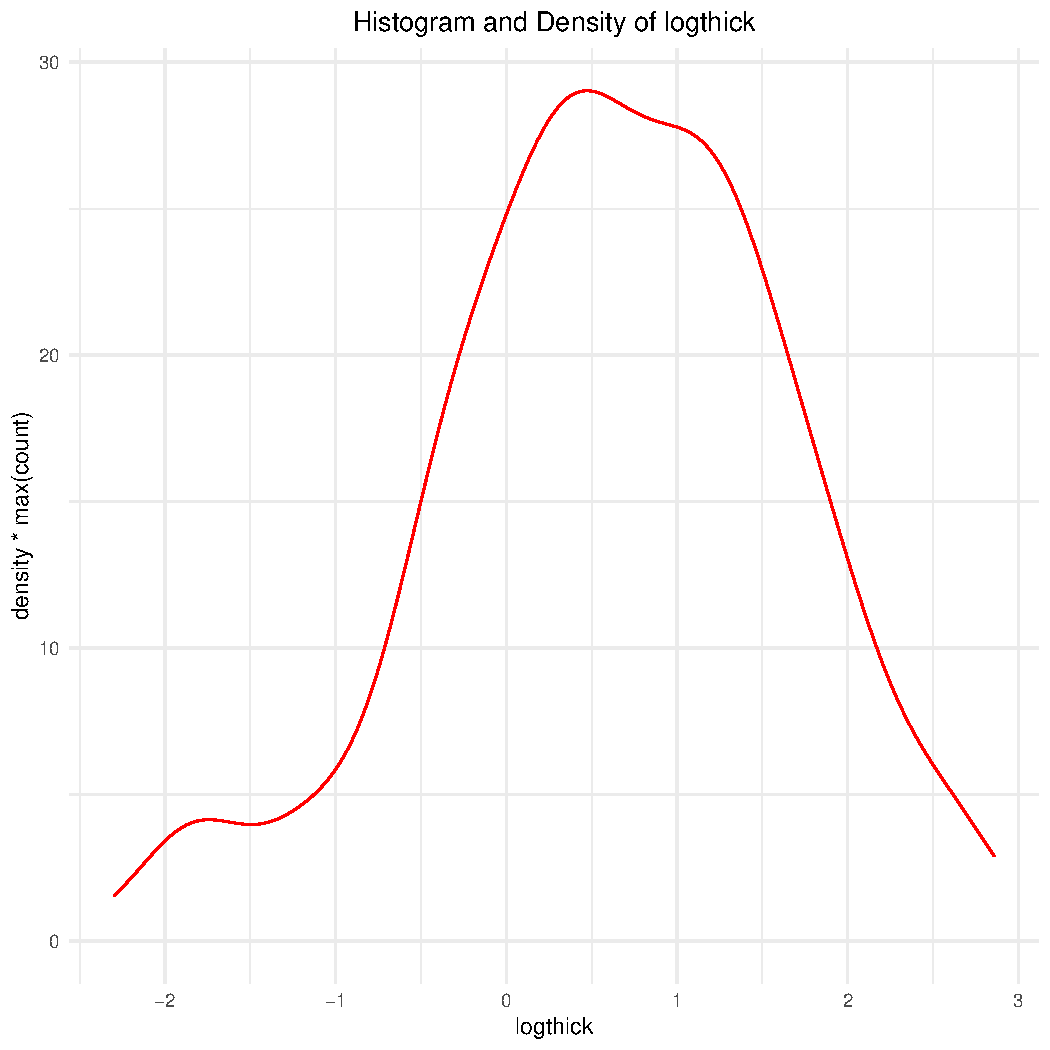
\includegraphics[width=\textwidth]{Basses_kode/Billeder_duration/Histogram_and_Density_of_ logthick .pdf} 
    \end{subfigure}
\end{figure}
\textbf{Outliers: }We see one outlier when taking log to it but to dertemin if the outlier has any influence on the health of the patient another method must be used aswell\\
\textbf{Distribution: }Kigges på distributionen af logaritmen af tykkelsen på tumor, vil der være en nogenlunde normaldistribution, dog med en tung venstre hale.
\item Depth of invasion of tumor score invas2.
\begin{table}[h!]
    \centering
    \begin{tabular}{|l|c|c|}
        \hline
        Invasion Level & Clark I-III & Clark IV-V \\
        \hline
        Count & 99 & 106 \\
        \hline
    \end{tabular}
    \caption{Counts by Invasion Level (Clark Staging)}
    \label{tab:invasion_level}
\end{table}

\end{enumerate}

Med henblik på de resterende, ikke kontinuerte variable, er der en fin distribution kategorierne imellem.



\chapter{3. Opgave}
I opgave 3 starter vi med at kigge på survival plottene. Den tydelige tendens er at jo højere kategori du tykkelsen befinder sig i, desto lavere overlevelses sandsynlighed har du. Altså har de personer med 20\% højest tykkelse en væsentlig lavere sandsynlighed for overlevelse end dem i 20\% tyndeste gruppe.\\
Når vi udfører en log-rank test ses det at vi får en p-værdi på 0.00001, hvilket er meget lavt. Dette indikerer dermed at der, som forventet, er stor forskel overlevelsessandsynlighed alt afhængigt af tykkelsen på tumor. Det er derfor samtidig retsvisende at antage at tumortykkelsen er en effektiv prediktor når overlevelses skal estimeres. Denne konklusion understøttes yderligere når man observerer survival plottene
\begin{figure}[h]
    \centering
    
\includegraphics[width=0.7\linewidth]{Basses_kode/Billeder_duration/Kaplan-Meier_Survival_Curves_by_Tumor_Thickness_Categories.pdf}
    \caption{Caption}
    \label{fig:enter-label}
\end{figure}


\chapter{4. Opgave}
Fitter man ved hjælp a Cox' opnås følgende:
\begin{table}[H]
\centering
\begin{tabular}{|l|c|}
\hline
\textbf{Variable} & \textbf{Coefficient} \\
\hline
age & 0.0231749 \\
thickness & 0.0006911 \\
epicellyes & -0.4106041 \\
ici & 0.2879794 \\
ulcerationyes & 0.8598251 \\
sexmale & 0.4557008 \\
invas2Clark IV-V & 0.1254010 \\
\hline
\end{tabular}
\caption{Coefficients for Variables}
\label{tab:coefficients}
\end{table}
I ovenstående tabel er der nogle fokuspunkter som observeres:\\
\textbf{epicellyes:} Her håndteres en kategorisk variabel hvor modellen er lavet udfra at resultatet "no" er baseline i modellen og dermed er det værdierne med "yes" som pålægges denne koefficient.\\
\textbf{ici:} ICI scoren er også en kategorisk parameter. Denne er dog anderledes i den forstand at den har inputs "1", "2", "3", "4", hvilket betyder at det pr. modellen er 4 gange så kritisk at have en ici score på 4 kontra en score på 1. Dette er ikke nødvendigvis retvisende og man kunne derfor argumenterer for om det havde været mere eksakt at give det værdierne "lav" "middel" "høj", "Meget høj" f.eks.\\
\textbf{ulcerationyes:} Denne er tilsvarende epicellyes, hvor "no" er baselineværdien.\\
\textbf{sexmale:} Denne er tilsvarende epicellyes, hvor "female" er baselineværdien.\\
\textbf{invas2ClarkIV-V:} Denne er tilsvarende epicellyes, hvor "Clark I-III" er baselineværdien.\\\\
Kigger man på martingale residualerne for alder ses en meget stabil kurve hvilket indikerer at der formentlig er en nogenlunde lineær sammenhæng mellem alder og overlevelses sandsynlighed. Dette i kombination med få outliers er incitament for ikke at det skulle være nødvendigt at transformere denne variabel.\\
Martingale residualerne for thickness er dog noget mere svingende. Her ser man afvigelser fra den lineære tendens hvilket kan skyldes flere ting. Først er det værd at bemærke at koefficienten for denne variabel $\approx 0$ hvilket kunne være relativt misvisende eftersom tykkelsen af tumor skulle have ret stor indflydelse på overlevelses sandsynligheden. Ydermere er der i thickness parameteren også en del outliers og en transformation (log, kvadratrod, el. lign) kan dermed være effektiv. Ved gennemgang af AIC for en model med en log transformeret thickness opnåes også en bedre AIC score hvilket vil blive berørt nærmere i spørgsmål 6.

\chapter{5. Opgave}





